% !TeX spellcheck = en_GB
\chapter{Maritime Communications and Operations}
\label{ch:maritime_background}
\lhead{Chapter \thechapter. \emph{\nameref{ch:maritime_background}}}

\section{Marine Operations, Payloads, Technologies, and Durations}\label{sec:marine_ops}

The use and applications of \glspl{auv} has undergone a great expansion in recent years~\cite{Alam2014}.
The primary application for \glspl{auv} has long been identified as the environmental monitoring of marine areas, and are actively being researched by a great range of industrial and defence sector applications, with secondary applications in the physical sciences and environmental research, which are summarised below~\cite{Bingham2002,Wynn2014}.

\subsection{\gls{auv} operations and deployments}

\subsubsection{Hydrographic Survey}

The use of \glspl{auv} in the place of manned-surface platforms or tethered undersea platforms enables greatly increased spatial and temporal sampling.
Importantly, the separation of \glspl{auv} from the noisy sea surface enables much more efficient survey operations.
This is particularly important when comparing to classical tow-line based measurements; where the mobility of the \glspl{auv} enables for much tighter-turning survey patterns or operation in inaccessible or hard-to-reach locations such as polar survey~\cite{Curtin1993}.

Another significant factor is cost; the daily cost of operating a manned vessel can be considerably higher than the costs of deploying, operating and recovering one or more \glspl{auv} with equivalent capabilities~\cite{Nicholson2008}.
Additionally, the use of low-power ``glider'' \glspl{auv} has lowered the barrier to entry for extended mission types, such as persistent environmental survey, or open-ocean operations. 
Depth-hardened \glspl{auv} have also opened up the deepest parts of the oceans to exploration, with onboard autonomy, imagery and \gls{slam} techniques allowing deep-dwelling survey \glspl{auv} to react to bottom-surface features without the need for a tight craft-to-surface control loop.
The natural extension of these kind of applications is the use of \glspl{auv} on ice-covered planets such as Europa, where three-dimensional, autonomous navigation without an on-the-loop controller is vital for mission resource efficiency and success.

\subsubsection{Hull and Infrastructure Inspection}
Ongoing concerns regarding the security, safety and legality of international shipping has driven the application of \glspl{auv} to the area of near-surface hull and infrastructure inspections, looking for damage as well as devices such as limpet mines and other contraband.
This use case puts a range of unique pressures on the \gls{auv} system; requiring highly accurate three-dimensional localisation and path-planning to clearly image the contours of a hull~\cite{Nicholson2008}.
Similarly, with the increasing use and criticality of intercontinental undersea optical fibre connections, using \glspl{auv} for both the laying of and inspection of these cables is an exciting area of work~\cite{Yu2004,Asakawa2002}.

\subsubsection{Marine Petrochemical/Mineralogy}
Oil and Gas industry requirements for high quality, low altitude bathymetry of seabed structures for infrastructure development (pipelines/drill platforms etc.) as well as monitoring of those structures over time (inspection etc.) is another significant application area, and a major driver of research investment.
As in Hydrography, the mobility of \glspl{auv} is the biggest single advantage over classical platforms~\cite{Morr2003}.
Additionally, recent advances in \gls{sas} have provided invaluable sub-surface profile data over much wider areas for multi-spectral mineralogical analysis than previous sonar profilers~\cite{Denny2015}.

\subsubsection{Military}
\gls{mcm} Operations benefit greatly from, and significantly drive, \gls{auv} development; the ability to rapidly explore and covertly survey a potentially dangerous area without risking a human operator is a major benefit both in Dedicated \gls{mcm} (e.g. Large Area Hunting/ \gls{eod} Clearance) and in Organic \gls{mcm} for Expeditionary Forces as well as general applications in  \gls{asw}, \gls{rea}, Navigational Aid and Force projection,
This benefit applies to protection as well as incursion; the ability to rapidly deploy persistent survey of a valuable area such as a forward-operating harbour is increasingly essential, and as \gls{auv} technology, autonomy and security practices develop, this use is increasing.
This Port Protection capability is particularly complex;  teams of \glspl{auv} are expected to repeatedly survey an area and remain densely-connected enough to maintain end-to-end communications with all other nodes, in the face of an environment that is possibly not well surveyed initially, and includes dynamically moving obstacles (i.e.\ ships).
As discussed in \autoref{sec:problem}, this Port Protection scenario is used as a baseline for our simulation context.


\subsection{Localisation Technologies}

Given the subsurface nature of most \gls{auv} operations, terrestrial localisation techniques such as \gls{gps} are unavailable (below $\approx 20cm$ depth). 
However, a range of alternative techniques are used to maintain spacial awareness to a high degree of accuracy in the underwater environment.
\subsubsection{\gls{lbl}}
Long-baseline localisation systems use a series of static surface/cable networked acoustic transponders to provide coordinated beacons and (usually) \gls{gps}-backed relative location information to local subsurface users. 
Such systems can be accurate to less that $0.\SI{1}{\meter}$ or better in ideal deployments and are regularly used in controlled autonomous survey environments such as harbour patrol operations where the deployment area is bounded. 
However, the initial set-up and deployment required in advance of any \gls{auv} operation makes \gls{lbl} difficult to utilise in unbounded or contended areas.
\gls{lbl} systems can also be deployed on mobile surface platforms in the area (ships or buoys for example), but these applications put significant computational pressure on the end-point AUV and have greatly reduced accuracy compared to ideal deployments~\cite{Matos1999}.
\subsubsection{\gls{dvl}}
Doppler Velocity Logging involves the emission of directed acoustic ``pings'' that reflect off sea bed/surface interfaces that, when received back on the craft with multi-beam phased array acoustic transducers can measure both the absolute depth/altitude (z-axis) of the craft and through directional Doppler shifting, the relative (xy-translative) motion of the craft since the ping.
While classical \gls{dvl} was highly sensitive to shifting currents in the water column, advances in the development of Acoustic Doppler Current Profiling has turned that situation on its head, enabling the compensation-for and measurement-of water currents down to the sub-meter level~\cite{Snyder2010}.
\subsubsection{\gls{ins}}
Inertial navigation systems use gyroscopic procession to observe the relative acceleration of a mobile platform.
This reference-relative monitoring is particularly useful in the underwater environment, as it detects the motion of \glspl{auv} as they are carried by the water itself.
Bias Drift is a significant problem for \glspl{ins} operating over longer (hundreds of metres) distances, as they usually have some minimal amount of directional bias, that incurs a cumulative effect over time without assistance.
Several sensor synthesis processes have been demonstrated which combine information from \gls{ins} along with \gls{dvl} data to improve localisation into the sub-decimeter level~\cite{Jalving2003,Liu2014,Allotta2015}.
\subsubsection{\gls{slam}}
Simultaneous Location and Mapping is the process of iteratively developing a feature-based model of an environment, and to use the relative movement within that modelled environment to obtain estimates of absolute positioning.
\gls{slam} has been most well developed in the contexts of either visual-based inspection using cameras, or LIDAR-style distance triangulation, however the same principles have been successfully applied using marine sonar readings, providing sub-meter accuracy, real-time, feature-relative localisation information that is (for the most part) environmentally agnostic~\cite{Williams2000}.

\vspace{\baselineskip}

In summary, current technology reliably enables \glspl{auv} to localise to a sub-metre accuracy in most areas of application.

\subsection{Example Maritime Autonomous Systems, Platforms and Operational Limitations}

\subsubsection{Kongsburg REMUS/HUGIN ranges}

The REMUS range of \gls{auv} platforms have been very popular in research and \gls{uan} application prototypes due to their relatively small size and high level of reconfigurability.
The basic configurations of the REMUS 100 configuration consist of a single pressure vessel, $\SI{0.2}{\meter}$ in diameter and $\SI{1.6}{\meter}$ long, weighting in at $37kg$, rated to operational depths of $\SI{150}{\meter}$. 
This package includes \gls{dvl}, \gls{ctd}, Underwater Videography, \gls{lbl} and onboard computing power suitable for low \gls{loa} independence, with onboard Li-on battery packs rated to provide up to 10-hours of cruising operational endurance.
These capabilities can be extended through the addition of further modular extensions through the REMUS range, such as the REMUS 600, rated for up to $\SI{600}{\meter}$ depth and a cruising endurance of 45 hours, or the REMUS 6000, rated for up to $\SI{6}{\kilo\meter}$ depth with 22 hours duration.

The HUGIN 1000 is a high-resolution extension to the REMUS range, characterised by it's default payload of a High Definition \gls{sas}, co-designed with the Norwegian Defence Research Establishment (FFI) for \gls{mcm} operations, with a dynamic depth rating up to $\SI{3}{\kilo\meter}$ and 24 hour cruising endurance (17 hours with continuous \gls{sas} engagement)

The Konsburg range also include range specific semi-automated \gls{lars}
\begin{figure}[h]
	\centering
	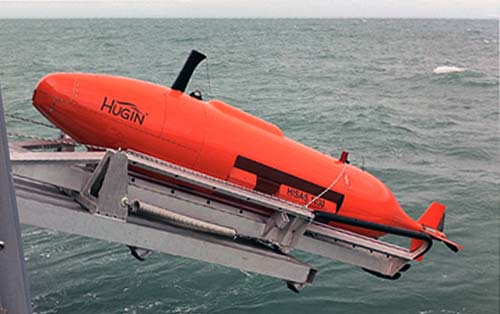
\includegraphics[width=0.45\textwidth]{hugin.jpg}
	\caption{\label{fig:hugin}HUGIN AUV mounted on LARS}
\end{figure}
\subsubsection{NOC Autosub}

Developed under the UK's National Oceanography Centres Marine Autonomous and Robotic Systems group, the Autosub family of \glspl{auv} is similar in many ways to the REMUS deployment profile; with long range and deep-ocean variants, operating at depths up to \SI{600}{\kilo\meter} for up to 36 hours (however, this configuration leaves it with a cruising speed of \SI{0.4}{\meter\per\second})
\begin{figure}[h]
	\centering
	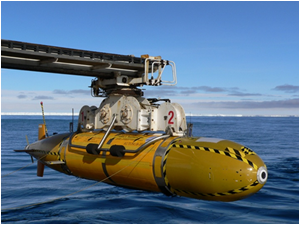
\includegraphics[width=0.45\textwidth]{autosub}
	\caption{\label{fig:autosub}NOC Autosub 3 being deployed off the Pine Island Glacier}
\end{figure}

\subsubsection{University of Washington SeaGlider}
Taking a fundamentally different approach to underwater mobility for targeting depth-variant environmental studies, the SeaGlider eschews classical propulsion to use it's downward-facing structure and fins to use it's weight/buoyancy to propel itself.   
At \SI{1.8}{\meter} long and weighing only \SI{52}{\kilogram}, this highly portable \gls{auv} can cover ranges up to \SI{4600}{\kilo\meter} with 650 \SI{1}{\kilo\meter} dive segments at a rate of \SI{0.25}{\meter\per\second}.
\begin{figure}[h]
	\centering
	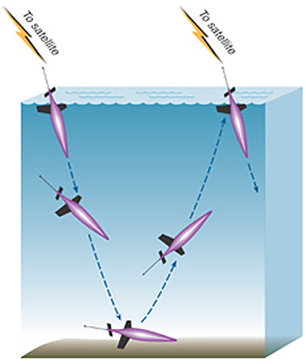
\includegraphics[width=0.45\textwidth]{seaglider}
	\caption{\label{fig:seaglider}''Flight path'' of the UW SeaGlider}
\end{figure}

\subsubsection{USN Sea Hunter}
The Sea Hunter is an autonomous unmanned surface vehicle (USV) launched in 2016 and is undergoing seatrials as part of the \gls{darpa} Anti-Submarine Warfare Continuous Trail Unmanned Vessel program, with a top speed of \SI{50}{\km\per\hour}, weighing \SI{122}{\tonne}.
While unarmed during its sea trials, the \emph{Sea Hunter} will be armed and used for \gls{asw} and \gls{mcm} duties, operating at a tiny fraction of the standard operating costs of a littoral destroyer.
\begin{figure}[h]
	\centering
	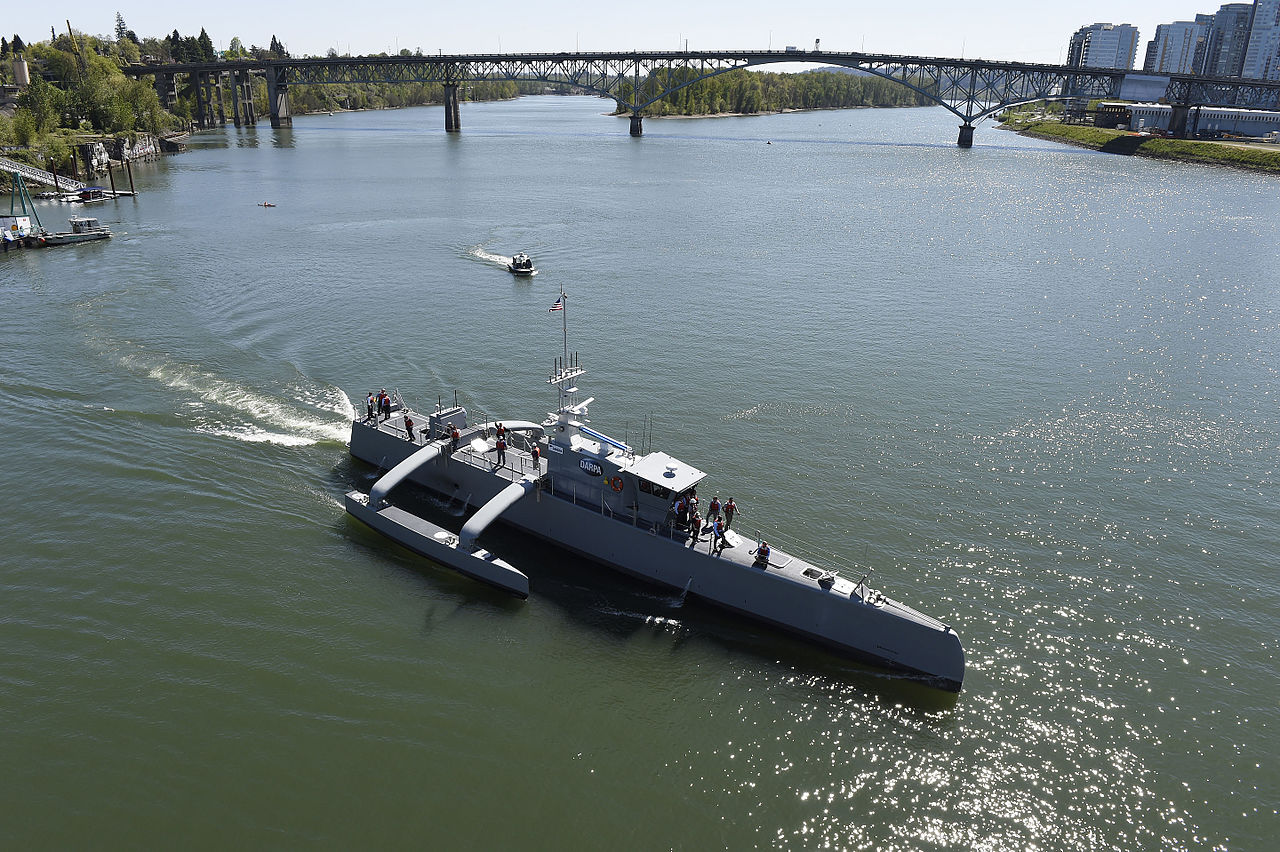
\includegraphics[width=0.45\textwidth]{seahunter}
	\caption[Initially manned deployment of the unmanned \emph{Sea Hunter}]{\label{fig:seahunter}Initially manned deployment of the unmanned \emph{Sea Hunter}. U.S. Navy photo by John F. Williams/Released}
\end{figure}

\subsection{Need for Trust in Maritime Networks}\label{sec:trust_in_marine}


Given the breadth of the threat space in \glspl{manet}, many strategies for mitigating these risks have been proposed in a matrix-basis; i.e. you can't cover all eventualities with one tool.
\autoref{tab:manet_risk} summaries some of these general strategies or ``solutions'' for range of threats identified specifically in the context of the deployment of \glspl{manet} in a tactical/defence context, originally based on~\citet{Kidston2010} but with some contextual alterations with modifications discussed below.

In this context of this table, Vulnerability is an assessment of how available a particular threat is to a generic attacker, Impact is an assessment of the in-system affects of a successful attack, and Risk is a qualitative assessment of the likelihood of exploitation of an attack.
\citet{Kidston2010} originally lowered the assessment of vulnerability of Eavesdropping to ``Low'', citing the tactical use of non-standard \gls{mac} as a barrier to attack, however considering the increasing commoditisation of tactical hardware across the world, and increasing application of \gls{cots} hardware, this is no longer a fair assessment.
Similarly, the assessment that the Risk of Data Corruption is low is arguable on the basis of simplistic spread spectrum jamming but this assessment is unchanged.
%Finally,~\citet{Kidston2010} did not take into account the presence of weapons or other actuation methods with \glspl{auv} as the endpoint.

\begin{table}
	\caption[Risks and Threat Mitigation Strategies for MANETs]{Risks and Threat Mitigation Strategies for \glspl{manet}, extended from~\citet{Kidston2010}}
	\label{tab:manet_risk}
	\begin{tabularx}{\textwidth}{p{3cm} X X X >{\raggedright\arraybackslash}p{4cm}}\toprule
		Threat & Vulnerability & Impact & Risk & Mitigation	\\\midrule
		Resource Depletion / \gls{dos} & Low-High & High & Low-High & Layer Specific Mechanisms~\cite{Wu2007,Nwaocha2015}\\
		Eavesdropping & Medium & High & Low & Cryptography~\cite{Chen2010}\\
		Masquerade & Low & Very High & Medium & Trust Systems and Cryptography~\cite{Wang2009a}\\
		Data Corruption & Low & High & Low & Cryptography\\
		Traffic Analysis & High & Low & Medium & Obfuscation~\cite{Huang2010}\\
		Misfire/Misactuation & Low & Very High & High & Man-in-the-loop firing~\cite{Caseley2009}\\
	\end{tabularx}
\end{table}

Resource Depletion, or \gls{dos} has a very wide ranging definition, from network-level attacks to saturate a communications channel or the computing resources of routing nodes, or the exploitation of a power-control loop to induce a node to waste energy with overly-high-powered communications, to the intentional geographic misleading of nodes to induce a similar power-drain on locomotive systems, through tactics such as location spoofing or \gls{gps} denial~\cite{Zuba2015}.

From \autoref{tab:manet_risk}, it is assessed that the highest overall threats are those of Resource Depletion and Masquerading.
Within this threat context, the general optimisation of any \gls{tmf} would be to prefer high but fair overall network throughput, while minimising delay, \gls{plr}, and power usage.

\subsection{Summary}

As \acrfull{auv} platforms become more capable and economical, they are being used in many applications requiring trust.
These applications are using the collective behaviour of teams or fleets of these \glspl{auv} to accomplish tasks~\cite{Caiti2011}, and this behaviour is increasingly being distributed across a network rather than being under direct, centralised, coordination~\cite{Korzun2015}.
With this use being increasingly isolated from stable communications networks, the establishment of trust between nodes is essential for the reliability and stability of such teams.

The use of Trust methods developed in the terrestrial \gls{manet} space will be re-appraised in \autoref{ch:comms_trust} for application within the challenging underwater communications channel.
That channel, and the appropriate modelling of it, is explored in the next section.
\pagebreak

\section{Maritime Communications Environment}\label{sec:marine_comms}

The key challenges of underwater acoustic communications are centred around the impact of slow and differential propagation of energy (RF, Optical, Acoustic) through water, and it's interfaces with the seabed / air.
The resultant challenges include; long delays due to propagation, significant inter-symbol interference and Doppler spreading, fast and slow fading due to environmental effects (aquatic flora/fauna; surface weather), carrier-frequency dependent signal attenuation, multipath caused by the medium interfaces at the surface and seabed, variations in propagation speed due to depth dependant effects (salinity, temperature, pressure, gaseous concentrations and bubbling), and subsequent refractive spreading and lensing due to that same propagation variation~\cite{Partan2006}.

\emph{Unless otherwise cited, formula and values for fundamental acoustic properties and models used in this section are taken from \citet{Urick1983}}

\subsection{Mechanics of Acoustic Transmission}

Unlike in RF energy transfer (where photons move through space to transmit energy from one place to another), acoustic waves are the result of mechanical perturbation of a medium where compressions and rarefactions pass energy across a medium\footnote{In essence, phased volumes of the medium (water) are put under instantaneous directed pressure, with the molecules of the medium moving a small distance away from the source of the compression wave. These in turn pressurise neighbouring molecules, continuing propagation forward and outward.}.
These ``compression waves'' propagate away from its source, and the rate of this propagation is the sound speed, velocity or $c$, measured in $ms^{-1}$.
This is not to be confused with the fluid velocity corresponding to the instantaneous motion of particles in the medium.

Hydrophones, like their more common microphone equivalent in air, are fundamentally pressure sensors.
Acoustic pressure is usually measured in \emph{Pascals} ($Pa/\mu Pa$). 
In the underwater environment, the dynamic range (difference between instantaneous high and low pressure values) may be extremely high, often more than 10 orders of magnitude higher. 
As such, logarithmic notation is justified.

Useful acoustic signals are generally maintained vibrations rather than instantaneous pulses.
They are characterised by their frequency $f$ expressed in Hertz ($Hz$) or by their Period ($T$) in seconds.
In commonly used underwater acoustics, used frequencies range from $\approx 10Hz-100kHz$ depending on application~\cite{Stojanovic2007}.

As with all waves, the relationship between frequency, period and the wavelength is given as in \autoref{eq:wavelength} where $c$ is the propagation speed in a given medium. 
As such the generally used upper and lower bounds of wavelength in most applications is from $\SI{1.5}{\meter} @ 10Hz$ to $\SI{0.015}{\meter} @ 100kHz$.
%
\begin{equation}
  \lambda = cT = \frac{c}{f}
  \label{eq:wavelength}
\end{equation}
%

This wide range of frequencies and wavelengths allow for a diverse set of constraining factors; (Paraphrased from~\citet{lurton2010}).

\begin{itemize}
  \item \emph{Attenuation} in water; limiting the maximum usable range, which increases very rapidly with frequency
  \item \emph{Dimensions} of sound source; which must be decreased as $f$ increases for a given transmission power
  \item \emph{Spatial Selectivity} of sources and receivers as $f$ increases, due to similarly increasing directivity of energy propagation.
  \item \emph{Acoustic Response} of target surfaces (analogous to receiver gain in RF networks).
\end{itemize}

\subsection{Velocity and density}\label{sec:aco_vel}

Air has a baseline density of approximately $\SI{1.3}{\kilogram\per\meter\cubed}$, and the speed of sound is typically static around $\SI{340}{\meter\per\second}$.
In sea water, acoustic wave velocity is close to $c=\SI{1500}{\meter\per\second}$ (generally between $\SIrange{1450}{1550}{\meter\per\second}$ depending on temperature, pressure, salinity etc.).
Similarly variable is sea water density, which is nominally $\rho = \SI{1027}{\kilogram\per\meter\cubed}$~\cite{Wang2010}.

While the sea/air surface is (ideally) a simple refractive interface, the interface between open seawater and marine sediment is graduated, with density ranging between $\SIrange{1200}{2000}{\kilogram\per\meter\cubed}$. 
This results in refractive and reflective velocities in the sediment interface ranging from $\SIrange{1500}{2000}{\meter\per\second}$~\cite{lurton2010}.
Additionally, depending on the relative buoyancy of different components of sediment in the water column, particularly fauna and biological/industrial sewage, there can be stratified sedimentary layers beyond the surface of the seabed, particularly in littoral and coastal shallow waters, that further complicate the characterisation of the density, and thus speed of sound, over the water column.

For comparison, the speed of light in air/water is $\SI{2.99e8}{\meter\per\second}$ and $\SI{2.249e8}{\meter\per\second}$ respectively. 

\begin{table}
	\centering
	\caption{Summary of physical factors differentiating terrestrial and acoustic channel constraints}
	\label{tab:channel_constraings_comp}
	\begin{tabularx}{0.8\textwidth}{X X X}\toprule
		Variable & Air & Water\\
		\midrule
		Density & $\SI{1.3}{\kilogram\per\meter\cubed}$ & $\approx\SI{1027}{\kilogram\per\meter\cubed}\pm0.5\%$ \\
		Speed of Sound & $\SI{340}{\meter\per\second}$ & $\approx\SI{1500}{\meter\per\second}\pm 5\%$ \\
		Speed of Light & $\SI{2.99e8}{\meter\per\second}$ & $\SI{2.249e8}{\meter\per\second}$\\
		\bottomrule
	\end{tabularx}
\end{table}
\citet{Mackenzie1981} proposed a more accurate model of acoustic velocity incorporating archival data from 15 worldwide sites that takes Temperature, Salinity and Depth into consideration.

\begin{align}
  c = & 1448.96 + 4.591 T - 5.304 \times 10^{-2} T^2 + 2.374 \times 10^{-4}T^{3}\notag\\
  & +1.340 (S-35) + 1.630\times 10^{-2}D+1.675\times 10^{-7}D^2\\
  & -1.025 \times 10^{-2}T(S-25) - 7.139\times 10^{-13}TD^3\notag
  \label{equ:mackenzie}
\end{align}

Where $T$ is the temperature in Celsius, $S$ the salinity in parts per thousand, and $D$ is the depth below the surface in meters.

\begin{figure}
	\centering
	\begin{subfigure}[t]{0.8\textwidth}
		\centering
		\includegraphics[width=\textwidth]{temp_globe}
		\caption{Surface Temperature}
		\label{fig:temp_globe}
	\end{subfigure}
	\begin{subfigure}[t]{0.8\textwidth}
		\centering
		\includegraphics[width=\textwidth]{sal_globe}
		\caption{Surface Salinity}
		\label{fig:sal_globe}
	\end{subfigure}
	\caption{Global Variations in selected Speed of Sound variance factors}
	\label{fig:globes}
\end{figure}

These are ``ideal'' assessments, and the parameters of this model are massively varied both across individual water columns, and indeed across bodies of water, across the world. 
\gls{noaa} regularly publish their \gls{woa}~\cite{Locarnini2013,Zweng2013} that includes these variables and many more, sampled across the world and at a range of depths. 
Outputs from these surveys are shown for example in \autoref{fig:globes}. 
Variability in Temperature across the globe is something that we are acutely aware of, but the significant regional variations, such as in the Sea of Japan, the US Eastern Seaboard, and between the Mediterranean and Black Seas (\autoref{fig:temp_globe}).
Global surface salinity appears almost uniform in comparison (\autoref{fig:sal_globe}).
However, a few global variants stand out, both due to the extremity of their transition in relatively small areas, and the general research / defence context of those areas. 
For example the differential between the geographically proximate and politically contentious Black, Caspian, and Mediterranean Seas, as well as the Persian Gulf exhibit variations from less than $6ppt$ to over $40ppt$.
Similarly, there is a navigable waterway providing access between the Baltic and North seas that across the $\SI{300}{\kilo\meter}$ long run from Malm{\"o} in Sweden to Skagen in Denmark, transitions from less than $5ppt$ to just under $30ppt$. 

Below the surface, the variability increases; \autoref{fig:temp_sal_profile} shows an example of a depth profile of these variations and the modelled impact on the speed of sound with respect to depth in three different regions. 
The variability of this speed is crucial to the operation of an underwater acoustic network, as it fundamentally changes the propagation paths of compressive energy transfer, and in particular, the fastest ``path''. 
\autoref{fig:ssps} shows the impact on this fastest received path and it's true path between two nodes in shallow, littoral, waters.
Even with relatively small variations in sound speed, and with the introduction of sea floor/surface interfaces, the ``fastest'' path deviates significantly from a true ``line of sight'' path where there is any variability in speed of sound profile, making delay-based positioning extremely difficult, and presents significant opportunities for out-of-sync multi-path effects\footnote{\autoref{fig:ssps} shows a staged, iterative approximation method to arrive at the shortest path, where the ``colour intensity'' of the chart shows the stage at which that path was explored, so the ``final'' paths are darkest, and the ``exploitative'' paths are lightest, however in reality these secondary paths are still emitted and arrive, delayed, to the receiver, causing significant inter-symbol interference unless equalised.}.

Recent work by \citet{Schmidt2016} further complicated the ocean-acoustic-comms field by showing that despite being one of the most studies areas of the world's oceans, the actual acoustic properties of the Beaufort Shelf have fundamentally changed in the past 20 years.
A thermally covalent subsurface acoustic channel has appeared that confounds modelling explanation but can provide a direct reliable acoustic path without surface/bed interfacing at a range of up to $\SI{\pm8}{\kilo\meter}$ away, or a near continuous (but noisy, due to surface ice interactions) to a range of $\SI{\pm80}{\kilo\meter}$.



\begin{figure}
	\centering
	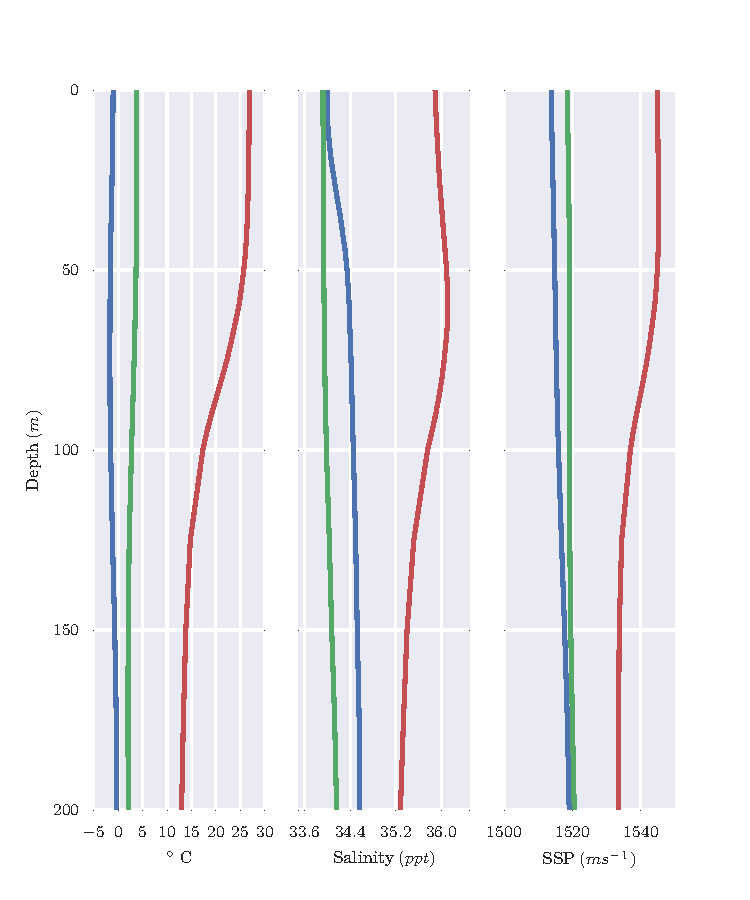
\includegraphics[height=6in]{temp_sal_profile}
	\caption{Depth Variations in selected Speed of Sound variance factors}
	\label{fig:temp_sal_profile}
\end{figure}


\begin{figure}
	\begin{subfigure}[t]{0.45\textwidth}
		\centering
		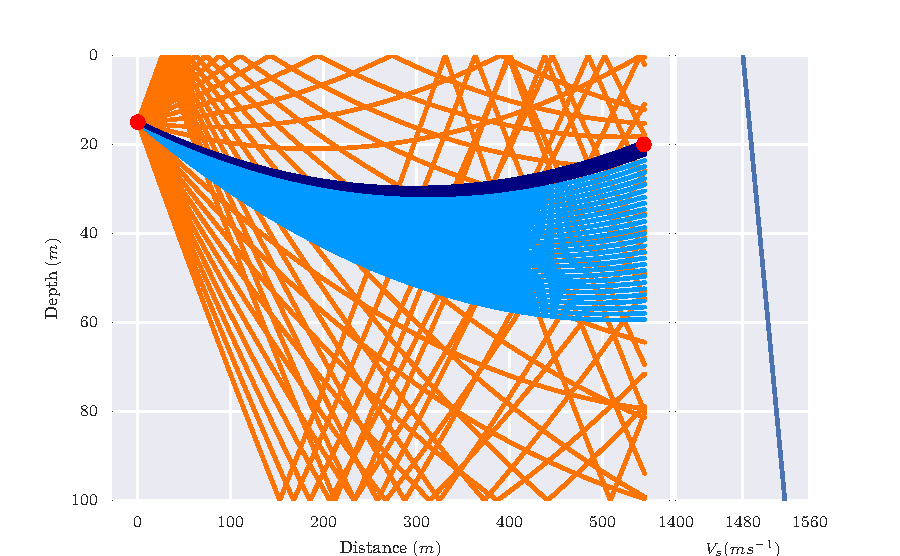
\includegraphics[width=\textwidth]{ssp_linear_increasing}
		\caption{Linear Increasing}
		\label{fig:ssp_linear_increasing}
	\end{subfigure}
	\begin{subfigure}[t]{0.45\textwidth}
		\centering
		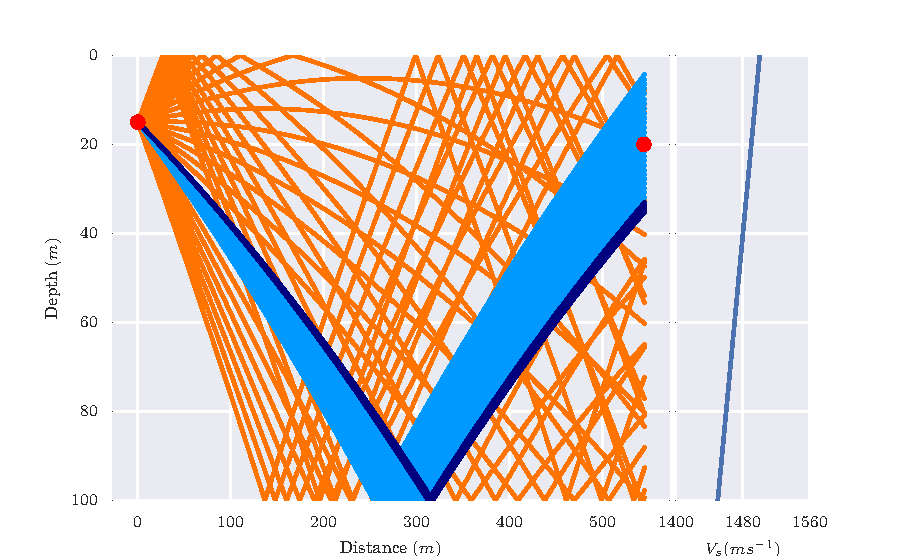
\includegraphics[width=\textwidth]{ssp_linear_decreasing}
		\caption{Linear Decreasing}
		\label{fig:ssp_linear_decreasing}
	\end{subfigure}\\
	\begin{subfigure}[t]{0.45\textwidth}
		\centering
		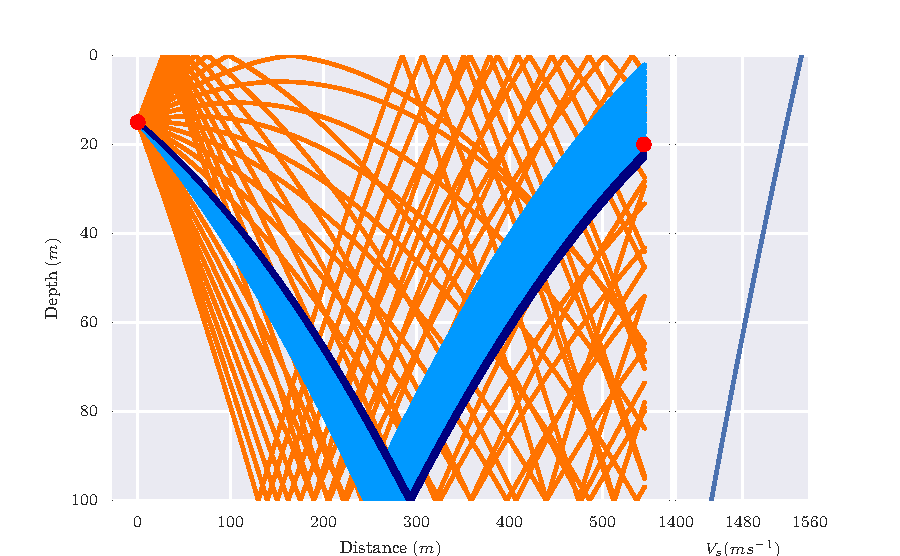
\includegraphics[width=\textwidth]{ssp_n_squared}
		\caption{Quadratic}
		\label{fig:ssp_n_squared}
	\end{subfigure}
	\begin{subfigure}[t]{0.45\textwidth}
		\centering
		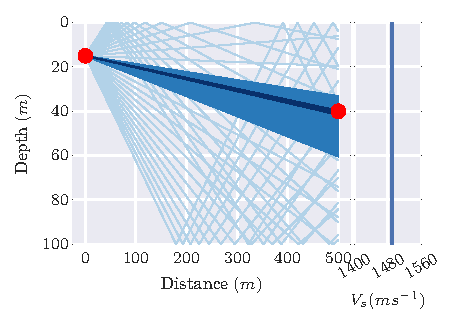
\includegraphics[width=\textwidth]{ssp_isovelocity}
		\caption{Isovelocity}
		\label{fig:ssp_isovelocity}
	\end{subfigure}
	\caption{Bellhop Model of Non-Linear Marine Shortest-Path Propagation in various Speed of Sound Profiles}
	\label{fig:ssps}
\end{figure}
\todo{Explain Fig:ssps}

\subsection{Intensity and Power} 

The energy of an acoustic wave is encapsulated into its kinetic and potential parts; where its kinetic energy corresponds to the active motion energy of the particles in the medium, and the potential energy corresponding to the elastic potential of the medium in displacement/compression.

The acoustic intensity ($I$) is the energy flux mean value per unit of surface and time \autoref{eq:acoustic_intensity} in Watts/$m^2$ where $p_0$ is the plane wave amplitude (pressure) and $P_{rms} = p_0/\sqrt{2}$

\begin{equation}
  I = \frac{p_0^2}{2\rho c} = \frac{p_{rms}^2}{\rho c}
  \label{eq:acoustic_intensity}
\end{equation}

\subsection{Attenuation}

The attenuation that occurs in an underwater acoustic channel over a distance $d$ for a signal about frequency $f$ in linear \autoref{eq:acoattenuation} and $dB$ forms \autoref{eq:acoattenuationdb} is given as;

\begin{equation}
  \label{eq:acoattenuation}
  A_{\text{aco}}(d,f) = A_0d^ka(f)^d
\end{equation}
\begin{equation}
  \label{eq:acoattenuationdb}
  10 \log A_{\text{aco}}(d,f)/A_0 = k \cdot 10 \log d + d \cdot 10 \log a(f)
\end{equation}

where $A_0$ is a unit-normalising constant, $k$ is a geometric spreading factor (commonly taken as 1.5 for practical use, but may be 2 for perfect spherical propagation or 1 for perfect plane-wave propagation)), and $a(f)$ is the absorption coefficient, that may be modelled in a variety of ways.

Thorp's formula (\autoref{eq:thorp}) is very simple, only depending on $f$, and is designed to be most accurate about a temperature of 4$^{\circ}$C at a depth of $\approx 1Km$.
%
\begin{figure}
  \begin{equation}
    10 \log a(f) = 0.11 \cdot \frac{f^2}{1+f^2} + 44\cdot\frac{f^2}{4100+f^2}+ 2.75\times10^{-4} f^2 + 0.003
    \label{eq:thorp}
  \end{equation}
  \caption[Thorp's formula]{Thorp's Absorption Model~\cite{Stojanovic2007}}
    \label{fig:thorp}
\end{figure}
%
The Ainslie \& McColm model is more complex, and incorporates the acidity of the water ($H^+$) as well as temperature ($T$), salinity ($S$ in parts per trillion) but not depth (\autoref{fig:ainslie}).
%
\begin{figure}
  \begin{align}
    10 \log a(f) =& 0.106 \frac{t_1 f^2}{t_1^2 + f^2} e^{\frac{H^+-8}{0.56}}\\\notag
      & + 0.52 \left(1+\frac{T}{43}\right)\left(\frac{S}{35}\right)\frac{t_2f^2}{t_2^2+f^2} e^{\frac{-D}{6}}\\\notag
      & + 4.9 \times 10^{-4} f^2e^{-\left(\frac{T}{27}+\frac{D}{17}\right)}\\\notag
      \text{Where}&\\\notag
      t_1 =& 0.78 \sqrt{\frac{S}{35}e^{\frac{T}{26}}}\\\notag
      t_2 =& 42 e^{\frac{T}{17}}\notag
      \label{eq:ainslie}
  \end{align}
  \caption{Ainslie \& McColm Absorption Model}
  \label{fig:ainslie}
\end{figure}
%
\begin{figure}
  \begin{align}
    10 \log a(f)=& A_1P_1\frac{t_1f^2}{t_1^2+f^2} + A_2P_2\frac{t_2f^2}{t_2^2+f^2} + A_3P_3f^2\\\notag
    \text{Where }&\\\notag
    A_1=&1.03\times 10^{-8} + 2.36\times 10^{-10} \cdot T -5.22 \times 10^{-12}\cdot T^2\\\notag
    A_2=&5.62\times 10^{-8} + 7.52\times 10^{-10} \cdot T\\\notag
    A_3=&\left(55.9 - 2.39\cdot T + 4.77\times 10^{-2}\cdot T^2 - 3.48 \times 10^{-4}\cdot T^3\right) \times 10 ^{-15}\\\notag
    t_1=&1.32\times 10^3\left(T+273.1\right)e^{\frac{-1700}{T+273.1}}\\\notag
    t_2=&1.55\times 10^7\left(T+273.1\right)e^{\frac{-3052}{T+273.1}}\\\notag
    P_1=&1\\\notag
    P_2=&\-10.3\times 10^{-4}\cdot P + 3.7\times 10^{-7}\cdot P^2\\\notag
    P_3=&\-3.84\times 10^{-4}\cdot P + 7.57\times 10^{-8}\cdot P^2\notag
    \label{eq:fisher}
  \end{align}
  \caption{Fisher-Simmons Absorption Model}
  \label{fig:fisher}
\end{figure}
%
The Fisher-Simmons model (\autoref{fig:fisher}) is significantly more complex, taking into account the effects of boric acid concentrations and dissolved magnesium sulphate. While there are several limitations on this model in terms of its being fixed at a salinity of 35 ppt and a pH of 8, as this model incorporates depth, temperature, distance and frequency, it is very attractive for research directed at high variability environments and is used for the remainder of this work unless otherwise stated.

%\todo{Possibly need to switch this with the Francois Garrison model which, depending on your source, is the refined version (or vise versa}



Regardless of the variations of particular attenuation models, comparing $A_{aco}(d,f)$ with the RF Free-Space Path Loss model~\autoref{eq:fspl}, the impact of range on signal power is exponential underwater, rather than quadratic in terrestrial RF ($A_{\text{aco}} \propto f^{2d}$ vs $A_{\text{RF}} \propto (df)^2$). 
While both frequency dependant factors are quadratic, approximating the factors in \autoref{eq:thorp}, $f\propto A_{\text{aco}}$ is at least 4 orders of magnitude higher than $f\propto A_{\text{RF}}$
\begin{equation}
  \label{eq:fspl}
  A_{\text{RF}}(d,f) \approx \left( \frac{4\pi d f}{c} \right)^2
  \text{where }c\approx \SI{3e8}{\meter\per\second}
\end{equation}


 \subsection{Ambient Noise Model}

 Historically, ambient ocean noise has be assumed to be Gaussian with a continuous power spectral density in dB re $\si{\micro\pascal\per\hertz}$, driven by four major factors, shown in \autoref{tab:ocean_noise_factors}, where $s$ is a shipping activity factor bounded from $[0,1]$ and $w$ is the surface wind speed in $\si{\meter\per\second}$~\cite{coates1989}.

\begin{table}[h]\centering
  \caption{Contributing factors to Ocean Ambient Acoustic Noise}
  \label{tab:ocean_noise_factors}
  \begin{tabularx}{\textwidth}{p{3.5cm} X}\toprule
    Source & Approximation \\ \midrule
    Turbulence & $10 \log N_t(f)=17-30\log f$\\
    Shipping & $10 \log N_s(f) = 40+20(s-0.5)+26\log f-60\log(f+0.03)$\\
    Wind Driven Waves & $10\log N_w(f) = 50+7.5w^{\frac{1}{2}}+20\log f - 40\log(f+0.4)$\\ 
    Thermal Noise & $10\log N_{th}(f) = \-15 + 20 log f$\\\bottomrule
  \end{tabularx}
\end{table}

However, recent work has cast doubt on this generalisation, and while a naive Gaussian model remains suitable and generally applicable for proof-of-concept work,  in real world applications, observed noise has several nigh frequency and impulsive components that must be taken into account~\cite{Mahmood2016, Deane2016}. 

\subsection{Multipath effects}

Refractive lensing and the multi-path nature of the medium result in line of sight propagation being extremely unreliable for estimating distances to targets (See \autoref{sec:aco_vel} and \autoref{fig:ssps}).
The first arriving acoustic signal has as the very least curved in the medium, and commonly has reflected off the surface/seabed before arriving at a receiver, creating secondary paths that are sometimes many times longer than the first arrival path, generating symbol spreading over orders of seconds depending on the ranges and depths involved.
Thus, the multi-path channel transfer function can be described by :

\begin{align}
  \label{eq:acomultipath}
  H(d,f) =\sum_{p=0}^{P-1} h(p) = \sum_{p=0}^{P-1} \Gamma_p / \sqrt{A(d_p,f)}e^{-j 2 \pi f \tau_p} \\
  \text{where } \tau_p = d_p/c, c \approx \SI{1500}{\meter\per\second} \notag
\end{align}

where $d=d_0$ is the minimal path length between the transmitter and receiver, $d_p,p=\{1,\dots P-1\}$ are the secondary path lengths, $\Gamma_p$ models additional losses incurred on each path such as reflection losses at the surface interface, and $\tau_p = d_p/c$ is the delay time.


\subsection{Modelling and Simulation of the Acoustic Medium / Channel}

Several toolkits exist in a that perform communications agent simulation, most notably the NS-2 / 3 family of frameworks and their add-ons.
Some of these frameworks, such as SUNSET~\cite{Petrioli2012a} and AquaTools~\cite{Sehgal2010}, that are particularly proven in their capability in modelling static network performance, with less in built support for advanced, reactive node mobilities such as those involving collision or object avoidance.

Beyond the NS family, there are many other communications and simulation modelling systems such as OpNet++~\cite{Chang1999} and MATLAB toolkits such as the AcTUP interface to the Ocean Acoustics Library, that primarily focus on simulation of the acoustic channel and contention issues without concentration on Underwater-specific \gls{mac} protocols.

AUVNetSim is a simulation platform designed from the ground up with collaborative \gls{auv} operations in mind~\cite{Miquel2008}.
Including support for dynamic modular mobility and application behaviours, considering the stated context of an environmentally reactive \gls{uan}, AUVNetSim was tested and selected as a foundation upon which to build an exploratory network testing framework for this research.

In order to implement a collaborative, reactive, simulation suite, the SimPy~\cite{Mueller2003SimPy} agent framework was used for ``background'' synchronisation.

As mentioned in the individual testing cases, transmission parameters for simulation were initially taken from and validated against results from~\citet{Stojanovic2007} and~\citet{Stefanov2011}.


\begin{comment}
\subsection{Routing and Network Design for \glspl{uan}}

Forward Error Correction coding is used on such channels to minimise packet losses.

\todo{ADD:Summary of Akyildiz02/05}

\todo{FIX:callback to routing discussion in c1 explain why fbr is the best of everything all the time}
\end{comment}
\pagebreak


%%%%%%%%%%%%%%%%%%%%%%%%%%%%%%%%%%%%%%%%%%%%%%%%%%%%%%%%%%%%%%%%%%%%%%%%%%%%%%%
